SŦYX supports functions which can have parameters and a return type.
The return type can be any of the supported data types.
Functions can be called from within the main function or other functions
and can be called recursively. They do not have to be defined in a specific order 
(except before the main function).\newline
At the current state of the language, the return statement does not immediately
stop the execution of the function, but instead returns the value to the caller
at the end of the function. The returned value from a function call can directly
be assigned to a variable of the same type or used as a parameter for another function call.
\newline
Here is some example code which shows the functions "foo" and "bar" and "main".
The function "main" has a print statement with the function call to "foo" as argument,
which itself has the integer 4 as argument. The function "foo" calls the function "bar",
which increments the given integer by 1 and returns it.
\begin{center}
    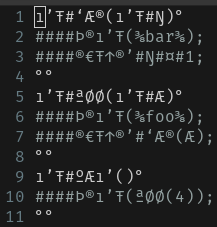
\includegraphics[width=0.3\textwidth]{styx_func.png}
\end{center}
